\documentclass[12pt]{article}

\usepackage{../discrete}

\usetikzlibrary{shapes}

\usepackage{pgf}

\heading{Math 228}{}{Advanced Counting Notes}



\begin{document}


\section{Stars and Bars}

Consider the following counting problem:

\begin{quote}
  You have 7 cookies to give to 4 kids.  How many ways can you do this?
\end{quote}

Take a moment to think about how you might solve this problem.  You may assume that it is acceptable to give a kid no cookies.  Also, the cookies are all identical.  And the order in which you give out the cookies does not matter.

Before solving the problem, here is a wrong answer.  You might guess that the answer should be $4^7$ because for each of the 7 cookies, there are 4 choices of kids to give the cookie too. This is reasonable, but wrong.  To see why, consider a few possible outcomes:  we could assign the first six cookies to kid A, and the seventh cookie to kid B.  Another outcome would assign the first cookie to kid B and the six remaining cookies to kid A.  Both outcomes are included in the $4^7$ answer.  But for our counting problem, both outcomes are really the same - kid A gets six cookies and kid B gets one cookie.

What do outcomes actually look like?  How can we represent them? One approach would be to write a outcome as a string of four numbers like this:
\[3112\]
which represent the outcome in which the first kid gets 3 cookies, the second and third kid each get 1 cookie, and the fourth kid gets 2 cookies.  Represented this way, the order in which the numbers occur matters - 1312 is a different outcome, because the first kid gets a one cookie instead of 3.  Each number in the string can be any integer between 0 and 7.  But the answer is not $7^4$ - we need the {\em sum} of the numbers to be 7.  

Another way we might represent outcomes is to write a string of seven letters:
\[\mbox{ABAADCD}\]
which represents that the first cookie goes to kid A, the second cookie goes to kid B, the third and fourth cookies go to kid A, and so on.  In fact, this outcome is identical to the previous one - A gets 3 cookies, B and C get 1 each and D gets 2.  Each of the seven letters in the string can be any of the 4 possible letters (one for each kid), but the number of such strings is not $4^7$, because here order does {\em not} matter.  In fact, another way to write the same outcome is
\[\mbox{AAABCDD}\]
This will be the preferred representation of the outcome.  Since we can write the letters in any order, we might as well write them in {\em non-decreasing} order for the purposes of counting.  So we will write all the A's first, then all the B's, and so on.  

Now think about how you could specify such an outcome.  All we really need to do is say when to switch from one letter to the next. In terms of cookies, we need to say after how many cookies do we stop giving cookies to the first kid and start giving cookies to the second kid.  And then after how many do we switch to the third kid?  And after how many do we switch to the fourth?  So yet another way to represent an outcome is like this:
\[***|*|*|**\]
Three cookies go to the first kid, then we switch and give one cookie to the second kid, then switch, one to the third kid, switch, two to the fourth kid.  Notice that we need 7 stars and 3 bars - one star for each cookie, and one bar for each switch between kids, so one fewer bars than there are kids (we don't need to switch after the last kid - we are done).

Why have we done all of this?  Simple: to count the number of ways to distribute 7 cookies to 4 kids, all we need to do is count how many {\em stars and bars} charts there are.  But a stars and bars chart is just a string of symbols, some stars and some bars.  If instead of stars and bars we would use 0's and 1's, it would just be a bit string.  We know how to count those.

Before we get too excited, we should make sure that really {\em any} string of (in our case) 7 stars and 3 bars corresponds to a different way to distribute cookies to kids.  In particular consider a string like this:
\[|***||****\]
Does that correspond to a cookie distribution?  Yes.  It represents the distribution in which kid A gets 0 cookies (because we switch to kid B before any stars), kid B gets three cookies (three stars before the next bar), kid C gets 0 cookies (no stars before the next bar) and kid D gets the remaining 4 cookies.  No matter how the stars and bars are arranged, we can distribute cookies in that way.  Also, given any way to distribute cookies, we can represent that with a stars and bars chart.  For example, the distribution in which kid A gets 6 cookies and kid B gets 1 cookie has the following chart:
\[******|*||\]

Now after all that work we are finally ready to count.  Each way to distribute cookies corresponds to a stars and bars chart with 7 stars and 3 bars.  So there are 10 symbols, and we must choose 3 of them to be bars.  Thus:
\[\mbox{ There are }{10 \choose 3}\mbox{ ways to distribute 7 cookies to 4 kids.}\]

While we are at it, we can also answer a related question: how many ways are there to distribute 7 cookies to 4 kids so that each kid gets at least one cookie?  What can you say about the corresponding stars and bars charts?  The charts must start and end with at least one star (so that kids A and D) get cookies, and also no two bars can be adjacent (so that kids B and C are not skipped).  One way to assure this is to only place bars in the spaces between the stars.  With 7 stars, there are 6 spots between the stars, so we must choose 3 of those 6 spots to fill with bars.  Thus there are ${6 \choose 3}$ ways to distribute 7 cookies to 4 kids giving at least one cookie to each kid.

Another (and more general) way to approach this modified problem is to first give each kid one cookie.  Now the remaining 3 cookies can be distributed to the 4 kids without restrictions.  So we have 3 stars and 3 bars for a total of 6 symbols, 3 of which must be bars.  So again we see that there are ${6 \choose 3}$ ways to distribute the cookies.



Stars and bars can be used in counting problems other than kids and cookies.  Here are a few examples.

\begin{example}
  Your favorite mathematical pizza chain offers 10 toppings.  How many pizzas can you make if you are allowed 6 toppings?  The order of toppings does not matter, but now you are allowed repeats - so one possible pizza is: triple sausage, double pineapple, and onions.
  \begin{solution}
    We get 6 toppings (counting possible repeats).  Represent each of these toppings as a star.  There are 10 toppings to choose from, so we must switch from considering one topping to the next 9 times - these are the bars.  Think of going down the menu one topping at a time: you see anchovies first, and skip to the next, sausage.  You say yes to sausage 3 times then switch to the next topping on the list.  You keep skipping until you get to pineapple, which you say yes to twice.  Another switch and you are at onions - you say yes once.  Then you keep switching until you get to the last topping, never saying yes again (since you already have said yes 6 times.
    
    Now that we are confident that we have the right number of stars and bars, we answer the question simply: there are 6 stars and 9 bars, so 15 symbols.  We need to pick 9 of them to be bars, so there number of pizzas possible is
    \[{15 \choose 9}\]
  \end{solution}
\end{example}


\begin{example}
  How many 7 digit phone numbers are there in which the digits are non-increasing?  That is, every digit is less than or equal to the previous one.


\begin{solution}
  We need to decide on 7 digits - so we will use 7 stars.  The bars will represent a switch from each possible single digit number down the next smaller one.  So the phone number 866-5221 is represented by the stars and bars chart
  \[|*||**|*|||**|*|\]
  There are 10 choices for each digit (0-9) so we must switch between choices 9 times.  We have 7 stars and 9 bars, so the total number of phone numbers is
  \[{16 \choose 9}\]
\end{solution}
\end{example}

\begin{example}
  How many integer solutions\footnote{An integer solution to an equation is a solution in which the unknown must have an integer value.} are there to the equation
  \[x_1 + x_2 + x_3 + x_4 + x_5 = 13\]
  \begin{enumerate}
    \item where $x_i \ge 0$ for each $x_i$?
    \item where $x_i > 0$ for each $x_i$?
    \item where $x_i \ge 2$ for each $x_i$?

  \end{enumerate}
  \begin{solution}
  This problem is just like giving 13 cookies to 5 kids - we need to say how many of the 13 units go to each of the 5 variables.  In other words, we have 13 stars and 4 bars (the bars are like the ``+'' signs in the equation).
      \begin{enumerate}
    \item If $x_i$ can be 0 or greater, we are in the standard case with no restrictions.  So 13 stars and 4 bars can be arranged in ${17 \choose 4}$ ways.
    \item Now each variable must be at least 1.  So give one unit to each variable to satisfy that restriction.  Now there are 8 stars left, and still 4 bars, so the number of solutions is ${12 \choose 4}$.
    \item Now each variable must be 2 or greater.  So before any counting, give each variable 2 free units.  We now have 3 remaining stars and 4 bars, so there are ${7 \choose 4}$ solutions.
      
  \end{enumerate}
  \end{solution}

\end{example}


\section{Functions}

Have we now discovered all the rules needed in counting?  Probably not.  To see what we can do and what we still must figure out, let's shift focus and think about counting in another way.  Consider again the problem if giving cookies to kids.  One way to think about this problem is to say that we are {\em assigning} each cookie to a kid.  Now in the case we have looked at so far, the cookies were identical, so it did not matter which cookie went to which kid.  But what if it did?  Suppose we have 7 different cookies and 4 different kids - how many ways are there to give out the cookies?

Perhaps you already have a solution in mind.  However, for the time being, we will consider this question more generally.  What are we really doing here?  We are {\em mapping} each cookie to a kid.  This sounds like a function!  It is.  To help us completely characterize counting problems, we should look at them as problems about how to count functions.  Before we proceed, here is a quick review of functions.

A function is simply a rule that assigns each input exactly one output.  The set of all inputs for a function is called the {\em domain}.  The set of all allowable outputs is called the codomain.  For example, a function might assign each natural number a natural number from 1 to 5.  In that case, the domain is the natural numbers and the codomain is the set of natural numbers from 1 to 5. Now it could be that this particular function we are thinking about assigns each even natural number to the number 2 and each odd natural number to the number 1.  In this case, not all of the codomain is actually used.  We would say that the set $\{1,2\}$ is the {\em range} of the function - these are the element in the codomain (allowable outputs) which are actually outputs for some input. 

The key thing that makes a rule assigning inputs to outputs a {\em function} is that there is {\em only one} output for an input.  In other words, it is important that the rule be a good rule.  What output do we assign to the input 7?  There can only be one answer for a particular function - otherwise where does 7 go to?  

To specify the name of the function, as well as the domain and codomain, we write $f:X \to Y$.  The function is called $f$, the domain is the set $X$ and the codomain is the set $Y$.  This however does not describe the rule.  To do that, we say something like this:

\begin{quote}
  The function $f:X \to Y$ is defined by $f(x) = x^2 + 3$.
\end{quote}

In this case, the function takes an input $x$ and computes the output by squaring $x$ and then adding 3.  In this case, you better hope that $X$ is a set of numbers and $Y$ is a set of number which can be 3 more than squares of numbers from $X$.  It would not work for $Y$ to be negative numbers here - that would not be a valid function.

The description of the rule can vary greatly.  If $X$ is a finite set, we might just give a list of each output for each input.  You could also describe the function with at able or a graph or in words.

\begin{example}
  The following are all examples of functions:
  \begin{enumerate}
    \item $f:\Z \to \Z$ defined by $f(n) = 3n$.  The domain and codomain are both the set of integers.  However, the range is only the set of integer multiples of 3.
    \item $f: \{1,2,3\} \to \{a,b,c\}$ defined by $f(1) = c$, $f(2) = a$ and $f(3) = a$.  The domain is the set $\{1,2,3\}$, the codomain is the set $\{a,b,c\}$ and the range is the set $\{a,c\}$.  Note that $f(2)$ and $f(3)$ are the same element of codomain.  This is not a problem - each element in the domain still has only one output (although each output does not have a unique input).
    \item $f:\{1,2,3\} \to \{1,2,3\}$ defined as follows:
    \begin{center}
      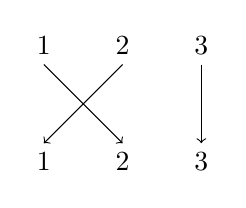
\begin{tikzpicture}
        \draw[->] (-1,1) node[above] {1} -- (0,0) node[below] {2};
        \draw[->] (0,1) node[above] {2} -- (-1,0) node[below] {1};
        \draw[->] (1,1) node[above] {3} -- (1,0) node[below] {3};
      \end{tikzpicture}

    \end{center}

  \end{enumerate}

\end{example}

The arrow diagram used to define the function above can be very helpful in visualizing functions.  We will often be working with functions on finite sets so this kind of picture is often more useful than a traditional graph of a function.  A graph of the function in example 3 above would look like this:

\begin{center}
  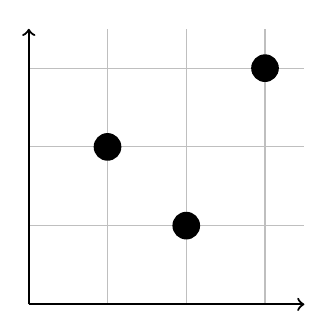
\begin{tikzpicture}
    %axis:
    \draw[thin, gray!50] (0,0) grid (3.5, 3.5);
    \draw[->, thick] (0,0) -- (0,3.5);
   \draw[->, thick] (0,0) -- (3.5,0);
   %points:
   \fill (1,2) circle (5pt) (2,1) circle (5pt) (3,3) circle (5pt);
  \end{tikzpicture}

\end{center}

It is important to know how to recognize a function from a rule which is not a function.  The arrow diagram can help.

\begin{example}
Which of the following diagrams represent a function.  Let $X = \{1,2,3,4\}$ and $Y = \{a,b,c,d\}$
  \begin{multicols}{3}
    \begin{center}
      $f:X \to Y$
      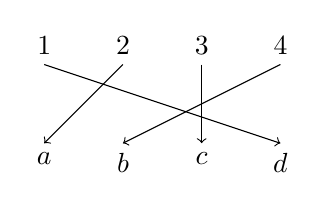
\begin{tikzpicture}
        \draw[->] (-1.5,1) node[above] {1} -- (1.5,0) node[below] {$d$};
        \draw[->] (-.5,1) node[above] {2} -- (-1.5,0) node[below] {$a$};
        \draw[->] (.5,1) node[above] {3} -- (.5, 0) node[below] {$c$};
        \draw[->] (1.5,1) node[above] {4} -- (-.5, 0) node[below] {$b$};
      \end{tikzpicture}
      \columnbreak
      
      $g:X \to Y$
	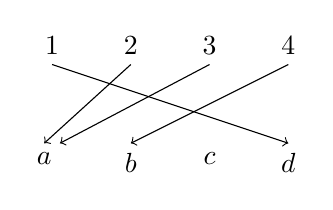
\begin{tikzpicture}
        \draw[->] (-1.5,1) node[above] {1} -- (1.5,0) node[below] {$d$};
        \draw[->] (-.5,1) node[above] {2} -- (-1.6,0) node[below] {$a$};
        \draw[->] (.5,1) node[above] {3} -- (-1.4, 0);
        \draw[->] (1.5,1) node[above] {4} -- (-.5, 0) node[below] {$b$};
        \draw (.5,0) node[below] {$c$};
      \end{tikzpicture}
      
      \columnbreak
      
      $h:X \to Y$
      	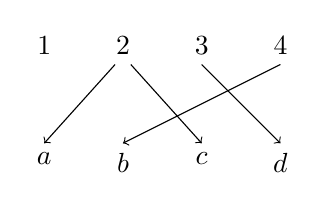
\begin{tikzpicture}
        \draw (-1.5,1) node[above] {1};
        \draw[->] (-.5,1) node[above] {2} (-.6,1) -- (-1.5,0) node[below] {$a$};
        \draw[->] (-.4,1) -- (.5,0);
        \draw[->] (.5,1) node[above] {3} -- (1.5, 0) node[below] {$d$};
        \draw[->] (1.5,1) node[above] {4} -- (-.5, 0) node[below] {$b$};
        \draw (.5,0) node[below] {$c$};
      \end{tikzpicture}
    \end{center}

  \end{multicols}
\begin{solution}
  $f$ is a function.  So is $g$.  There is no problem with an element of the codomain not being the output for any input, and there is no problem with $a$ from the codomain being the output of both 2 and 3 from the input.  
  
  However, $h$ is {\bf not} a function - in fact, for two reasons.  First, the element 1 from the domain has not been mapped to any element from the codomain.  Second, the element 2 from the domain has been mapped to more than one element from the codomain ($a$ and $c$).  Note that either one of these problems is enough to make a rule not a function.  Neither of these mappings are functions:
  \begin{center}
    \begin{multicols}{2}
      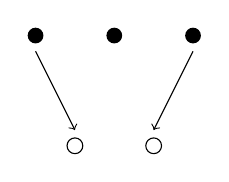
\begin{tikzpicture}
        \fill (-1, 1.2) circle (.1) (0,1.2) circle (.1) (1, 1.2) circle (.1);
        \draw[->] (-1, 1) -- (-.5,0);
        \draw[->] (1,1) -- (.5, 0);
        \draw (-.5, -0.2) circle (.1) (.5, -0.2) circle (.1);
      \end{tikzpicture}
       
       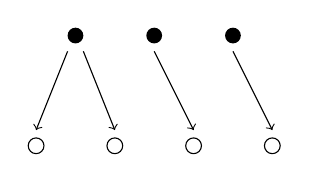
\begin{tikzpicture}
         \fill (-1, 1.2) circle (.1) (0,1.2) circle (.1) (1, 1.2) circle (.1);
         \draw[->] (-1.1, 1) -- (-1.5, 0);
         \draw[->] (-.9, 1) -- (-.5, 0);
         \draw[->] (0,1) -- (.5,0);
         \draw[->] (1,1) -- (1.5, 0);
         \draw (-.5, -0.2) circle (.1) (.5, -0.2) circle (.1) (-1.5, -0.2) circle (.1) (1.5, -0.2) circle (.1);
       \end{tikzpicture}

    \end{multicols}
  Not functions.
  \end{center}

\end{solution}

\end{example}

\subsection{Surjections, Injections, and Bijections}

We now turn to investigating special properties functions might or might not possess.  

In the examples above, you may have noticed that sometimes there are elements of the codomain which are not in the range - which are not actual outputs for any input.  When this sort of the thing {\em does not} happen, (that is, when everything in the codomain is in the range) we say the function is {\em onto} or that the function maps the domain {\em onto} the codomain.  This terminology should make sense: the function puts the domain (entirely) on top the codomain.  The fancy math term for an onto function is a {\em surjection}, and we say that an onto function is a {\em surjective} function.

In pictures:

\begin{multicols}{2}
  \begin{center}
          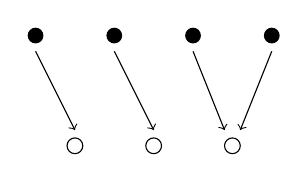
\begin{tikzpicture}
        \fill (-1.5, 1.2) circle (.1) (-.5,1.2) circle (.1) (.5, 1.2) circle (.1) (1.5,1.2) circle (.1);
        \draw[->] (-1.5, 1) -- (-1,0);
        \draw[->] (-.5,1) -- (0, 0);
        \draw[->] (.5, 1) -- (.9,0);
        \draw[->] (1.5,1) -- (1.1,0);
        \draw (-1, -0.2) circle (.1) (0, -0.2) circle (.1) (1, -0.2) circle (.1);
      \end{tikzpicture}
      
      Surjective
      
      \columnbreak
      
                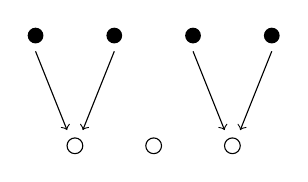
\begin{tikzpicture}
        \fill (-1.5, 1.2) circle (.1) (-.5,1.2) circle (.1) (.5, 1.2) circle (.1) (1.5,1.2) circle (.1);
        \draw[->] (-1.5, 1) -- (-1.1,0);
        \draw[->] (-.5,1) -- (-.9, 0);
        \draw[->] (.5, 1) -- (.9,0);
        \draw[->] (1.5,1) -- (1.1,0);
        \draw (-1, -0.2) circle (.1) (0, -0.2) circle (.1) (1, -0.2) circle (.1);
      \end{tikzpicture}
      
      Not surjective
  \end{center}

\end{multicols}

\begin{example}
  Which functions are surjective (i.e., onto)?
    \begin{enumerate}
    \item $f:\Z \to \Z$ defined by $f(n) = 3n$.  
    \item $g: \{1,2,3\} \to \{a,b,c\}$ defined by $g(1) = c$, $g(2) = a$ and $g(3) = a$.  
    \item $h:\{1,2,3\} \to \{1,2,3\}$ defined as follows:
    \begin{center}
      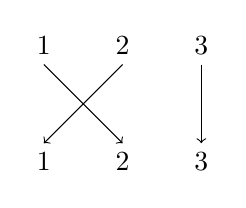
\begin{tikzpicture}
        \draw[->] (-1,1) node[above] {1} -- (0,0) node[below] {2};
        \draw[->] (0,1) node[above] {2} -- (-1,0) node[below] {1};
        \draw[->] (1,1) node[above] {3} -- (1,0) node[below] {3};
      \end{tikzpicture}
    \end{center}
  \end{enumerate}
  \begin{solution}
    \begin{enumerate}
      \item $f$ is not surjective.  There are elements in the codomain which are not in the range.  For example, no $n \in \Z$ gets mapped to the number 1 (the rule would say that $\frac{1}{3}$ would be sent to 1, but $\frac{1}{3}$ is not in the domain).  In fact, the range of the function is $3\Z$ (the integer multiples of 3), which is not equal to $\Z$.
      \item $g$ is not surjective.  There is no $x \in \{1,2,3\}$ (the domain) for which $g(x) = b$.  So $b$, which is in the codomain, is not in the range, so once again the function is not onto.
      \item $h$ is surjective.  Every element of the codomain is also in the range.  Nothing is missed.
    \end{enumerate}

  \end{solution}

\end{example}


To be a function, a map cannot assign a single element of the domain to two or more different elements of the codomain.  However, we have seen that the reverse is permissible.  That is, a function might assign the same element of the codomain to two or more different elements of the domain.  When this {\em does not} occur - that is, when each element of the codomain is assigned to at most one element of the domain - then we say the function is {\em one-to-one}.  Again, this terminology makes sense: we are sending at most one element from the domain to one element from the codomain.  One input to one output. The fancy math term for a one-to-one function is a {\em injection}.  We call one-to-one functions {\em injective} functions.

In pictures:

\begin{multicols}{2}
  \begin{center}
          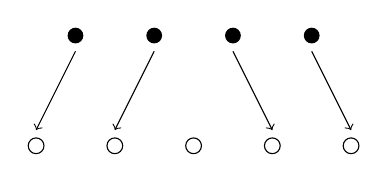
\begin{tikzpicture}
        \fill (-1.5, 1.2) circle (.1) (-.5,1.2) circle (.1) (.5, 1.2) circle (.1) (1.5,1.2) circle (.1);
        \draw[->] (-1.5, 1) -- (-2,0);
        \draw[->] (-.5,1) -- (-1, 0);
        \draw[->] (.5, 1) -- (1,0);
        \draw[->] (1.5,1) -- (2,0);
        \draw (-2, -0.2) circle (.1) (-1, -.2) circle (.1) (0, -0.2) circle (.1) (1, -0.2) circle (.1) (2, -0.2) circle (.1);
      \end{tikzpicture}
      
      Injective
      
      \columnbreak
      
                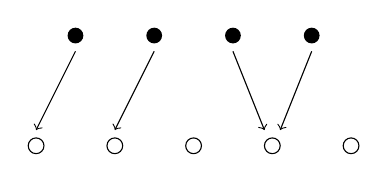
\begin{tikzpicture}
        \fill (-1.5, 1.2) circle (.1) (-.5,1.2) circle (.1) (.5, 1.2) circle (.1) (1.5,1.2) circle (.1);
        \draw[->] (-1.5, 1) -- (-2,0);
        \draw[->] (-.5,1) -- (-1, 0);
        \draw[->] (.5, 1) -- (.9,0);
        \draw[->] (1.5,1) -- (1.1,0);
        \draw (-2, -0.2) circle (.1) (-1, -.2) circle (.1) (0, -0.2) circle (.1) (1, -0.2) circle (.1) (2, -0.2) circle (.1);
      \end{tikzpicture}
      
      Not injective
  \end{center}

\end{multicols}


\begin{example}
  Which functions are injective (i.e., one-to-one)?
    \begin{enumerate}
    \item $f:\Z \to \Z$ defined by $f(n) = 3n$.  
    \item $g: \{1,2,3\} \to \{a,b,c\}$ defined by $g(1) = c$, $g(2) = a$ and $g(3) = a$.  
    \item $h:\{1,2,3\} \to \{1,2,3\}$ defined as follows:
    \begin{center}
      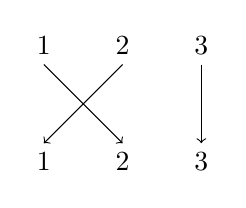
\begin{tikzpicture}
        \draw[->] (-1,1) node[above] {1} -- (0,0) node[below] {2};
        \draw[->] (0,1) node[above] {2} -- (-1,0) node[below] {1};
        \draw[->] (1,1) node[above] {3} -- (1,0) node[below] {3};
      \end{tikzpicture}
    \end{center}
  \end{enumerate}
  \begin{solution}
    \begin{enumerate}
      \item $f$ is injective.  Each element in the codomain is assigned to at {\em most} one element from the domain - if $x$ is a multiple of three, then only $x/3$ is mapped to $x$.  If $x$ is not a multiple of 3, then there is no input corresponding to the output $x$.
      \item $g$ is not injective.  Both inputs $2$ and $3$ are assigned the output $a$.
      \item $h$ is injective.  Each output is only an output once.
    \end{enumerate}

  \end{solution}

\end{example}



From the examples above, it should be clear that there are functions which are surjective, injective, both or neither.  In the case when a function is both one-to-one and onto (a injection and surjection) we say the function is a {\em bijection}, or that the function is a {\em bijective} function.  

\begin{defbox}{Function Definitions}
\vspace{-2em}
\begin{itemize}
  \item A {\em function} is a rule that assigns each element of a set, called the {\em domain}, to exactly one element of a second set, called the {\em codomain}.
  \item Notation: $f:X \to Y$ is our way of saying that the function is called $f$, the domain is the set $X$ and the codomain is the set $Y$.
  \item $f(x) = y$ means the element $x$ of the domain (input) is assigned to the element $y$ of the codomain.  We say $y$ is an output.  Alternatively, we call $y$ the {\em image of $x$ under $f$}.
  \item The {\em range} is a subset of the codomain.  It is the set of all elements which are assigned to at least one element of the domain by the function.  That is, the range is the set of all outputs.
  \item A function is {\em one-to-one} (also called an {\em injection}) if every element of the codomain is the output for \textbf{at most} one element from the domain.
  \item A function is {\em onto} (also called a {\em surjection}) if every element of the codomain is the output of \textbf{at least} one element of the domain.
  \item A {\em bijection} is a function which is both an injection and surjection - so one-to-one and onto.
%  \item The {\em complete inverse image} of an element in the codomain, written $f\inv(y)$ is the {\bf set} of all element in the domain which are assigned to $y$ by the function.  
\end{itemize}

\end{defbox}

\subsection{Counting Functions}

Now back to counting.  Suppose (yet again) that you have 7 cookies to give to 4 kids.  Now the cookies are all different, so which cookie goes to which kid matters.  How many ways are there to do this?  What we really have is a function with domain the set of cookies and codomain the set of kids.  So we might as well ask:

\begin{example}
 How many functions are there $f: \{1,2,3,4,5,6,7\} \to \{a,b,c,d\}$?
 \begin{solution}
 	We must assign $f(x)$ for each $x$ in the domain.  We have four choices for $f(1)$ - we could have $f(1) = a$, $f(1) = b$, $f(1) = c$ or $f(1) = d$.  Similarly, we have four choices for $f(2)$, and four choices for $f(3)$ and so on.  In fact, for each of the seven elements of the domain, we have four choices, so the number of functions here is $4^7$.  
 \end{solution}
\end{example}

We might also wonder how many of those functions are injective and how many are surjective.  What would these mean in terms of cookies?  The function would be injective if each kid got no more than one cookie.  There is no way to do this, because we have more cookies than kids.  The number of injective functions with this domain and codomain is 0.  What if we switch the domain and codomain?  So now we are mapping kids to cookies.  Note that this is not the same, although it is a perfectly fine counting question (the answer is $P(7,4)$, do you see why?). 

On the other hand, a surjective function would be one in which each kid got at least one cookie.  Can we count those? It turns out that counting surjective functions is hard.  We will do it, but first back up and consider another simpler example.

\begin{example}
  How many functions are there $f: \{1,2,3,4,5\} \to \{a,b,c,d,e\}$?  How many of those functions are injective? 
  \begin{solution}
    First we count all the functions with domain $\{1,2,3,4,5\}$ and codomain $\{a,b,c,d,e\}$.  For $f$ to be a function, it must assign each element of the domain to exactly one element of the codomain.  In other words, we need to assign one of the elements of $\{a,b,c,d,e\}$ to $f(1)$.  There are 5 choices for this.  Similarly, there are five choices for $f(2)$.  In fact, there are 5 choices for $f(x)$ for all five possible values of $x \in \{1,2,3,4,5\}$.  Thus the total number of function is $5 \cdot 5 \cdot 5 \cdot 5 \cdot 5 = 5^5$.
    
    What about the injective (one-to-one) functions?  Again, we have 5 choices for $f(1)$.  However, once we assign a value to $f(1)$, we cannot assign that value to $f(2)$, or any other $f(x)$.\footnote{Remember, a function is injective if and only if different elements from the domain go to {\em different} elements of the codomain.} So for each of the 5 choices for $f(1)$, we only have 4 choices for $f(2)$, and then only 3 choices for $f(3)$ and only 2 choices for $f(4)$, leaving only 1 choice (the last element of the codomain) for $f(5)$.  Therefore the number of one-to-one functions is $5!$.
  \end{solution}

\end{example}

Using the same counting techniques, you should be able to count the total number of functions from any finite size domain to any finite size codomain, and also count the one-to-one functions (as long as the size of the codomain is at least as large as the domain, otherwise there would be no one-to-one functions).

So what about surjective functions?  Well in the previous example, there are exactly $5! = 120$ surjections.  We know this because whenever the domain and codomain of a function are the same finite size, a function is injective if and only if it is surjective.  In general, if the domain and codomain both contain $n$ elements, then the number of surjective functions is $n!$, since this is the number of injective functions.  Also, if the codomain is strictly larger than the domain, then the surjective functions are easy to count - there are 0 of them (since there will always be elements of the codomain left out of the range).  But what if the size of the codomain is smaller than the size of the domain?

The idea is to count the functions which are {\em not} surjective, and them subtract that from the total number of functions.  This works very well when the codomain has two elements in it.

\begin{example}
  How many functions $f: \{1,2,3,4,5\} \to \{a,b\}$ are surjective?
  \begin{solution}
    There are $2^5$ functions all together - there are two choices for where to send each of the 5 elements of the domain.  Now of these, the functions which are {\em not} surjective must exclude one or more elements of the codomain from the range.  So first, consider functions for which $a$ is not in the range.  This can only happen one way - everything gets sent to $b$.  Alternatively, we could exclude $b$ from the range.  Then everything gets sent to $a$, so there is only one function like this.  These are the only ways in which a function could not be onto (no function excludes both $a$ and $b$ from the range) so there are exactly $2^5 - 2$ surjective functions.
  \end{solution}
\end{example}

When there are three elements in the codomain, there are now three choices for a single element to exclude from the range.  Additionally, we could pick pairs of two elements to exclude from the range, and we must make sure we don't over count these.

\begin{example}
  How many functions $f: \{1,2,3,4,5\} \to \{a,b,c\}$ are surjective?
  \begin{solution}
   Again start with the total number of functions: $3^5$ (as each of the five elements of the domain can go to any of three elements of the codomain).  Now we count the functions which are {\em not} surjective.
   
   Start by excluding $a$ from the range.  Then we have two choices ($b$ or $c$) for where to send each of the five elements of the domain.  Thus there are $2^5$ functions which exclude $a$ from the range.  Similarly, there are $2^5$ functions which exclude $b$, and another $2^5$ which exclude $c$.  Now have we counted all functions which are not surjective?  Yes, but in fact, we have counted some multiple times.  For example, the function which sends everything to $c$ was one of the $2^5$ functions we counted when we excluded $a$ from the range, and also one of the $2^5$ functions we counted when we excluded $b$ from the range.  We must subtract out all the functions which specifically exclude two elements from the range.  There is 1 function when we exclude $a$ and $b$, one function when we exclude $a$ and $c$, and one function when we exclude $b$ and $c$.  
   
   We are using PIE: to count the functions which are not surjective, we added up the functions which exclude $a$, $b$, and $c$ separately, then subtracted the functions which exclude pairs of elements.  We would then add back in the functions which exclude groups of three elements, except that there are no such functions.  We find that the number of functions which are {\em not} surjective is
   \[2^5 + 2^5 + 2^5 - 1 - 1 - 1 + 0\]
   Perhaps a more descriptive way to write this is
   \[{3 \choose 1}2^5 - {3 \choose 2}1^5 + {3 \choose 3}0^5\]
   since each of the $2^5$'s was the result of choosing 1 of the 3 elements of the codomain to exclude from the range, each of the three $1^5$'s was the result of choosing 2 of the 3 elements of the codomain to exclude.  Writing $1^5$ instead of 1 makes sense too: we have 1 choice of were to send each of the 5 elements of the domain.
   
   Now we can finally count the number of surjective functions:
   \[3^5 - \left[{3 \choose 1}2^5 - {3 \choose 2}1^5\right] = 150\]
  \end{solution}

\end{example}

You might worry that to count surjective functions when the codomain is larger than 3 elements would be too tedious - we need to use PIE but with more than 3 sets the formula for PIE is very long.  However, we have lucked out.  As we saw in the example above, the number of functions which exclude a single element from the range is the same no matter which single element is excluded.  Similarly, the number of functions which exclude a pair of elements will be the same for every pair.  With larger codomains, we will see the same behavior with groups of 3, 4, and more elements excluded.  So instead of adding/subtracting each of these, we can simply add or subtract all of them at once, if you know how many there are.  Here's what happens with $4$ and $5$ elements in the codomain.

\begin{example}
  \begin{enumerate}
    \item How many functions $f: \{1,2,3,4,5\} \to \{a,b,c,d\}$ are surjective?
    \item How many functions $f: \{1,2,3,4,5\} \to \{a,b,c,d,e\}$ are surjective?
  \end{enumerate}
\begin{solution}
  \begin{enumerate}
    \item There are $4^5$ functions all together - we will subtract the functions which are not surjective.  We could exclude any one of the four elements of the codomain, and doing so will leave us with $3^5$ functions.  This counts too many so we subtract the functions which exclude two of the four elements of the codomain, each pair giving $2^5$ functions.  But this excludes too many, so we add back in the functions which exclude three of the four elements of the codomain, each triple giving $1^5$ function.  There are ${4 \choose 1}$ groups of functions excluding a single element, ${4 \choose 2}$ groups of functions excluding a pair of elements, and ${4 \choose 3}$ groups of functions excluding a triple of elements.  This means that the number of functions which are {\em not} surjective is:
    \[{4 \choose 1}3^5 - {4 \choose 2}2^5 + {4 \choose 3}1^5\]
    We can now say that the number of functions which are surjective is:
    \[4^5 - \left[{4 \choose 1}3^5 - {4 \choose 2}2^5 + {4 \choose 3}1^5\right]\]
    
    \item The number of surjective functions is:
    \[5^5 - \left[{5 \choose 1}4^5 - {5 \choose 2}3^5 + {5 \choose 3}2^5 - {5 \choose 4}1^5\right]\]
    We took the total number of functions $5^5$ and subtracted all that were not surjective.  There were ${5 \choose 1}$ ways to select a single element from the codomain to exclude from the range, and for each there were $4^5$ functions.  But this double counts, so we use PIE and subtract functions excluding two elements from the range: there are ${5 \choose 2}$ choices for the two elements to exclude, and for each pair, $3^5$ functions.  This takes out too many functions, so we add back in functions which exclude 3 elements from the range: ${5 \choose 3}$ choices for which three to exclude, and then $2^5$ functions for each choice of elements.  Finally we take back out the 1 function which excludes 4 elements for each of the ${5 \choose 4}$ choices of 4 elements.
  \end{enumerate}

\end{solution}

\end{example}


\section{Advanced Counting using PIE}

Counting surjections used the Principle of Inclusion/Exclusion (PIE), which gives a method for finding the cardinality of the union of not necessarily disjoint sets. The idea is that to find how many things are in {\em one or more} of the sets $A$, $B$, and $C$ we should just add up the number of things in each of these sets.  However, if there is any overlap among the sets, those elements are counted multiple times.  So we subtract the things in each intersection of a pair of sets.  But doing this removes elements which are in all three sets once too often, so we need to add it back in.

For four or more sets, we do not write down a formula for PIE.  Instead, we just think of the principle: add up all the elements in single sets, then subtract out things you counted twice (elements in the intersection of a {\em pair} of sets), then add back in elements you removed too often (elements in the intersection of groups of three sets), then take back out elements you added back in too often (elements in the intersection of groups of four sets), then add back in, take back out, add back in, etc.  

Here are some additional examples of how it can be used.

\subsection{Counting Derangements}

A {\em derangement} of $n$ elements $\{1,2,3,\ldots, n\}$ is a permutation in which no element is fixed.  For example, there are $6$ permutations of the three elements $\{1,2,3\}$:
\[123 ~~ 132 ~~ 213 ~~ 231 ~~ 312 ~~ 321\]
but most of these have one or more elements fixed: $123$ has all three elements fixed, $132$ has the first element fixed (1 is in its original first position), and so on.  In fact, the only derangements of three elements are
\[231 \mbox{  and  }312\]
If we go up to 4 elements, there are 24 permutations (because we have 4 choices for the first element, 3 choices for the second, 2 choices for the third leaving only 1 choice for the last - $4! = 24$).  How many of these are derangements?  If you list out all 24 permutations and eliminate those which are not derangements, you will be left with just 9 derangements.  Let's see how we can get that number using PIE.

\begin{example}
  How many derangements are there of 4 elements?
  \begin{solution}
    We count all permutations, and subtract those which are not derangements.  There are $4! = 24$ permutations of 4 elements.  Now for a permutation to {\em not} be a derangement, at least one of the 4 elements must be fixed.  There are ${4 \choose 1}$ choices for which single element we fix.  Once fixed, we need to find a permutation of the other three elements - there are $3!$ permutations on 3 elements.  But now we have counted too many non-derangements, so we must subtract those permutations which fix two elements.  There are ${4 \choose 2}$ choices for which two elements we fix, and then for each pair, $2!$ permutations of the remaining elements.  But this subtracts too many, so add back in permutations which fix 3 elements, all ${4 \choose 3}1!$ of them.  Finally subtract the ${4 \choose 4}0!$ permutations (recall $0! = 1$) which fix all four elements.  All together we get that the number of derangements of 4 elements is:
    \[4! - \left[{4 \choose 1}3! - {4 \choose 2}2! + {4 \choose 3} 1! - {4 \choose 4}0!\right] = 24 - 15 = 9\]
    
  \end{solution}

\end{example}

Of course we can use a similar formula to count the derangements on any number of elements.  However, the more elements we have, the longer the formula gets.  It turns out that there is no closed formula for counting derangements or surjective functions for that matter.  We need to use PIE.  

Before moving on to another advanced counting technique, here is another example.

\begin{example}
  Five gentlemen attend a party, leaving their hats at the door.  At the end of the party, they hastily grab hats on their way out.  How many different ways could this happen so that none of the gentlemen leave with their own hat?
  
  \begin{solution}
    We are counting derangements on 5 elements.  There are $5!$ ways for the gentlemen to grab hats in any order - but many of these permutations will result in someone getting their own hat.  So we subtract all the ways in which one or more of the men get their own hat.  In other words, we subtract the non-derangements. Doing so requires PIE.  Thus the answer is:
    
    \[5! - \left[{5 \choose 1}4! - {5 \choose 2}3! + {5 \choose 3}2! - {5 \choose 4}1! + {5 \choose 5}0!\right]\]
  \end{solution}

\end{example}

\subsection{Stars, Bars, and Pie}

Another time PIE crops up is in stars and bars problems.  Let's go back to our 7 cookies and 4 kids problem.  Recall we want to distribute the 7 identical cookies to 4 (non-identical) kids.  Now we place a restriction on it

\begin{example}
How many ways can you distribute 7 cookies to 4 kids so that no kid gets more than 2 cookies?  

\begin{solution}
To answer this, we will subtract all the outcomes in which a kid gets 3 or more cookies.  How many outcomes are there like that?  We can force kid A to eat 3 or more cookies by giving him 3 cookies before we start.  Doing so reduces the problem to one in which we have 4 cookies to give to 4 kids without any restrictions.  In that case, we have 4 stars (the 4 remaining cookies) and 3 bars (one less than the number of kids) so we can distribute the cookies in ${7 \choose 3}$ ways.  Of course we could choose any one of the 4 kids to give too many cookies, so it would appear that there are ${4 \choose 1}{7 \choose 3}$ ways to distribute the cookies giving too many to one kid.  But in fact, we have over counted.  We must get rid of the outcomes in which two kids have too many cookies.  There are ${4 \choose 2}$ ways to select to 2 kids to give extra cookies.  It takes 6 cookies to do this, leaving only 1 cookie.  So we have 1 star and still 3 bars.  The remaining 1 cookie can thus be distributed in ${4 \choose 3}$ ways (for each of the ${4 \choose 2}$ choices of which 2 kids to over-feed).  We could continue in this fashion (using PIE) but there are no ways to give too many cookies to 3 kids - you don't have enough cookies.

All together we get that the number of ways to distribute 7 cookies to 4 kids without giving any kid more than 2 cookies is:
\[{10 \choose 3} - \left[{4 \choose 1}{7 \choose 3} - {4 \choose 2}{4 \choose 3}\right] = 120 - [ 140 - 24] = 4\]
This makes sense: the only way to distribute cookies with this restriction is for 3 kids to get 2 cookies and one kid to get 1.  There are 4 choices for which kid gets the 1 cookie.
\end{solution}
\end{example}


\begin{example}
Earlier we counted the number of solutions to the equation
\[x_1 + x_2 + x_3 + x_4 + x_5 = 13.\]

How many of those solutions have $0 \le x_i \le 3$ for each $x_i$? 


\begin{solution}
 We must subtract off the number of solutions in which one or more of the variables has a value greater than 3.  We will need to use PIE because counting the number of solutions for which each of the five variables separately are greater than 3 counts solutions multiple times.  Here is what we get:
    \begin{itemize}
      \item Total solutions: ${17 \choose 4}$
      \item Solutions where $x_1 > 3$: ${13 \choose 4}$ - give $x_1$ 4 units first, then distribute the remaining 9 units to the 5 variables.
      \item Solutions where $x_1 > 3$ and $x_2 > 3$: ${9 \choose 4}$ - after you give 4 units to $x_1$ and another 4 to $x_2$, you only have 5 units left to distribute.
      \item Solutions where $x_1 > 3$, $x_2 > 3$ and $x_3 > 3$: ${5 \choose 4}$.
      \item Solutions where $x_1 > 3$, $x_2 > 3$, $x_3 > 3$, and $x_4 > 3$: 0.
    \end{itemize}
    We also need to account for the fact that we could choose any of the five variables in the place of $x_1$ above, any pair of variables in the place of $x_1$ and $x_2$ and so on.  It is because of this that the double counting occurs, so we need to use PIE.  All together we have that the number of solutions with $0 \le x_i \le 3$ is
    \[{17 \choose 4} - \left[{5\choose 1}{13 \choose 4} - {5 \choose 2}{9 \choose 4} + {5 \choose 3}{5 \choose 4}\right]\]
  \end{solution}
\end{example}




%7 cookies for 4 kids:  In other words, you are giving a function with domain the cookies and codomain the kids - assigning each cookie to a kid. 





% You have probably already tried a problem like the following:
%
%\begin{example}
%  How many $8$-bit strings of weight 5 either start with $11$ or end with $01$ (or both)?
%  \begin{solution}
%    First consider all $8$-bit strings of weight 5 which start with $11$.  After these first two bits, we still need 6 bits, and of these 3 of them must be 1's (so that the total weight is 5).  There are ${6 \choose 3}$ such strings.  Therefore the {\em set} of $8$-bit strings of weight 5 starting with 11 has cardinality ${6 \choose 3} = 20$.
%    
%    Next consider the set of $8$-bit strings of weight $5$ which end with $01$.  There are 6 other bits, and 4 of them must be 1's, so there are ${6 \choose 4} = 15$ strings in this set.
%    
%    Now to answer the main question.  We want to know how many strings are in the first or second set (or both) described above.  The principle of inclusion/exclusion says that the answer should be \[20 + 15 - \mbox{(the number of strings in both sets)}.\]  So what is the size of the intersection?  Strings in the intersection must have $8$ bits, $5$ of them need to be 1's, and they must start with 11 and end with 01.  There are 4 other bits to determine, and 2 of them must be 1's, so there are ${4 \choose 2}$ strings in the intersection. Therefore the total number of $8$-bit strings of weight 5 which start with 11 or end with 01 is
%    \[{6 \choose 3} + {6 \choose 4} - {4 \choose 2} = 20 + 15 - 6 = 29\]
%  \end{solution}
%
%\end{example}


\end{document}


